\documentclass[14pt]{extbook}
\usepackage{multicol, enumerate, enumitem, hyperref, color, soul, setspace, parskip, fancyhdr} %General Packages
\usepackage{amssymb, amsthm, amsmath, bbm, latexsym, units, mathtools} %Math Packages
\everymath{\displaystyle} %All math in Display Style
% Packages with additional options
\usepackage[headsep=0.5cm,headheight=12pt, left=1 in,right= 1 in,top= 1 in,bottom= 1 in]{geometry}
\usepackage[usenames,dvipsnames]{xcolor}
\usepackage{dashrule}  % Package to use the command below to create lines between items
\newcommand{\litem}[1]{\item#1\hspace*{-1cm}\rule{\textwidth}{0.4pt}}
\pagestyle{fancy}
\lhead{Progress Quiz 3}
\chead{}
\rhead{Version C}
\lfoot{3148-2249}
\cfoot{}
\rfoot{Spring 2021}
\begin{document}

\begin{enumerate}
\litem{
Write the equation of the line in the graph below in Standard form $Ax+By=C$. Then, choose the intervals that contain $A, B, \text{ and } C$.
\begin{center}
    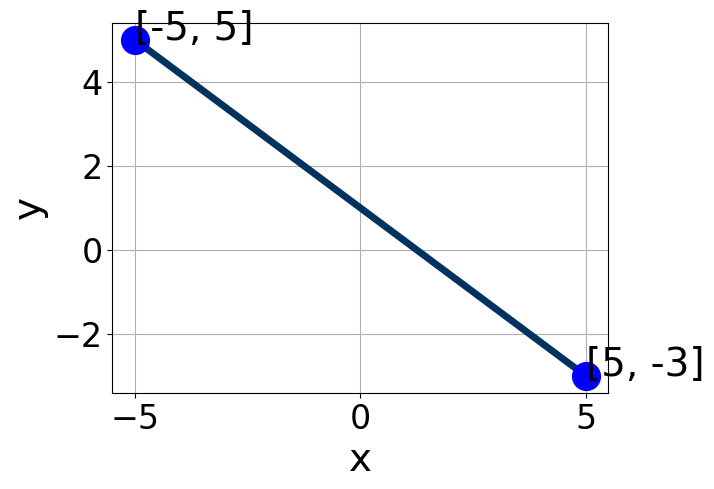
\includegraphics[width=0.5\textwidth]{../Figures/linearGraphToStandardCopyC.png}
\end{center}
\begin{enumerate}[label=\Alph*.]
\item \( A \in [-0.4, 1.6], \hspace{3mm} B \in [-3.2, 0.5], \text{ and } \hspace{3mm} C \in [-2.9, 0.2] \)
\item \( A \in [2.1, 6.3], \hspace{3mm} B \in [-6, -4], \text{ and } \hspace{3mm} C \in [-6.5, -3.9] \)
\item \( A \in [-4.8, -3.1], \hspace{3mm} B \in [-6, -4], \text{ and } \hspace{3mm} C \in [-6.5, -3.9] \)
\item \( A \in [-0.4, 1.6], \hspace{3mm} B \in [0.9, 3], \text{ and } \hspace{3mm} C \in [-0.9, 1.5] \)
\item \( A \in [2.1, 6.3], \hspace{3mm} B \in [3.9, 5.9], \text{ and } \hspace{3mm} C \in [3.3, 7.8] \)

\end{enumerate} }
\litem{
Solve the equation below. Then, choose the interval that contains the solution.\[ -5(6x -12) = -10(2x + 13) \]\begin{enumerate}[label=\Alph*.]
\item \( x \in [-3.4, 0.6] \)
\item \( x \in [4, 9] \)
\item \( x \in [-7, -4] \)
\item \( x \in [19, 21] \)
\item \( \text{There are no real solutions.} \)

\end{enumerate} }
\litem{
Solve the equation below. Then, choose the interval that contains the solution.\[ -2(3x + 14) = -19(-9x -6) \]\begin{enumerate}[label=\Alph*.]
\item \( x \in [-0.82, -0.73] \)
\item \( x \in [-0.65, -0.49] \)
\item \( x \in [0.43, 0.52] \)
\item \( x \in [-0.5, -0.42] \)
\item \( \text{There are no real solutions.} \)

\end{enumerate} }
\litem{
Find the equation of the line described below. Write the linear equation as $ y=mx+b $ and choose the intervals that contain $m$ and $b$.\[ \text{Perpendicular to } 5 x + 8 y = 3 \text{ and passing through the point } (9, 3). \]\begin{enumerate}[label=\Alph*.]
\item \( m \in [1.3, 3.1] \hspace*{3mm} b \in [-15.4, -7.4] \)
\item \( m \in [-0.8, 1.2] \hspace*{3mm} b \in [-15.4, -7.4] \)
\item \( m \in [-3, 0.1] \hspace*{3mm} b \in [17.4, 20.4] \)
\item \( m \in [1.3, 3.1] \hspace*{3mm} b \in [10.4, 14.4] \)
\item \( m \in [1.3, 3.1] \hspace*{3mm} b \in [-6, -5] \)

\end{enumerate} }
\litem{
Find the equation of the line described below. Write the linear equation as $ y=mx+b $ and choose the intervals that contain $m$ and $b$.\[ \text{Perpendicular to } 9 x + 4 y = 12 \text{ and passing through the point } (4, -2). \]\begin{enumerate}[label=\Alph*.]
\item \( m \in [-0.32, 0.68] \hspace*{3mm} b \in [3.1, 6.5] \)
\item \( m \in [1.58, 2.49] \hspace*{3mm} b \in [-4.6, -0.6] \)
\item \( m \in [-0.32, 0.68] \hspace*{3mm} b \in [-7.2, -4.5] \)
\item \( m \in [-0.32, 0.68] \hspace*{3mm} b \in [-4.6, -0.6] \)
\item \( m \in [-0.71, -0.02] \hspace*{3mm} b \in [-1.1, -0.1] \)

\end{enumerate} }
\litem{
First, find the equation of the line containing the two points below. Then, write the equation as $ y=mx+b $ and choose the intervals that contain $m$ and $b$.\[ (7, -5) \text{ and } (-9, 9) \]\begin{enumerate}[label=\Alph*.]
\item \( m \in [-0.7, 3] \hspace*{3mm} b \in [16.57, 17.98] \)
\item \( m \in [-2.1, 0.8] \hspace*{3mm} b \in [0.88, 1.19] \)
\item \( m \in [-2.1, 0.8] \hspace*{3mm} b \in [-12.48, -10.75] \)
\item \( m \in [-2.1, 0.8] \hspace*{3mm} b \in [-1.96, 0.76] \)
\item \( m \in [-2.1, 0.8] \hspace*{3mm} b \in [17.02, 18.34] \)

\end{enumerate} }
\litem{
Write the equation of the line in the graph below in Standard form $Ax+By=C$. Then, choose the intervals that contain $A, B, \text{ and } C$.
\begin{center}
    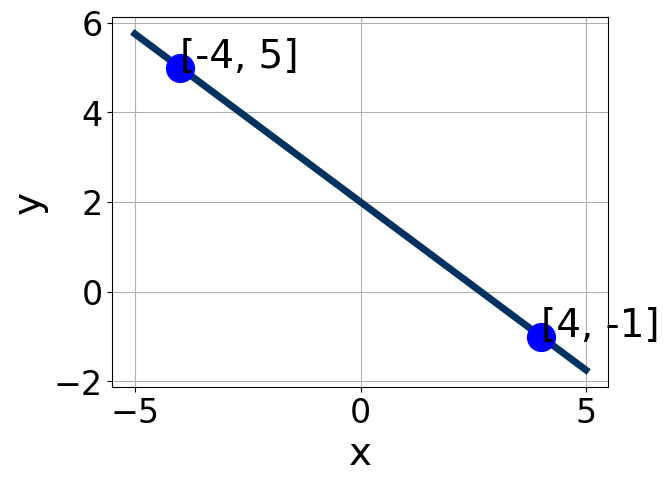
\includegraphics[width=0.5\textwidth]{../Figures/linearGraphToStandardC.png}
\end{center}
\begin{enumerate}[label=\Alph*.]
\item \( A \in [2.24, 3.02], \hspace{3mm} B \in [-4.2, -3.44], \text{ and } \hspace{3mm} C \in [-12, -7] \)
\item \( A \in [-0.48, 0.84], \hspace{3mm} B \in [-1.95, 0.23], \text{ and } \hspace{3mm} C \in [-2, 1] \)
\item \( A \in [-4.64, -2.13], \hspace{3mm} B \in [-4.2, -3.44], \text{ and } \hspace{3mm} C \in [-12, -7] \)
\item \( A \in [-0.48, 0.84], \hspace{3mm} B \in [0.13, 1.5], \text{ and } \hspace{3mm} C \in [2, 4] \)
\item \( A \in [2.24, 3.02], \hspace{3mm} B \in [3.72, 4.68], \text{ and } \hspace{3mm} C \in [7, 14] \)

\end{enumerate} }
\litem{
Solve the linear equation below. Then, choose the interval that contains the solution.\[ \frac{-9x + 9}{8} - \frac{-5x -8}{6} = \frac{-3x -4}{2} \]\begin{enumerate}[label=\Alph*.]
\item \( x \in [-17.38, -15.38] \)
\item \( x \in [3.46, 9.46] \)
\item \( x \in [-4.69, -1.69] \)
\item \( x \in [-3.48, 1.52] \)
\item \( \text{There are no real solutions.} \)

\end{enumerate} }
\litem{
Solve the linear equation below. Then, choose the interval that contains the solution.\[ \frac{-8x + 7}{5} - \frac{-5x -3}{3} = \frac{5x -8}{6} \]\begin{enumerate}[label=\Alph*.]
\item \( x \in [4, 7.3] \)
\item \( x \in [1.9, 2.6] \)
\item \( x \in [0.3, 0.7] \)
\item \( x \in [21.3, 24.9] \)
\item \( \text{There are no real solutions.} \)

\end{enumerate} }
\litem{
First, find the equation of the line containing the two points below. Then, write the equation as $ y=mx+b $ and choose the intervals that contain $m$ and $b$.\[ (6, -7) \text{ and } (3, -4) \]\begin{enumerate}[label=\Alph*.]
\item \( m \in [-0.4, 3.8] \hspace*{3mm} b \in [-8.2, -6.35] \)
\item \( m \in [-2.8, 0.1] \hspace*{3mm} b \in [-1.34, -0.58] \)
\item \( m \in [-2.8, 0.1] \hspace*{3mm} b \in [-13.05, -12.42] \)
\item \( m \in [-2.8, 0.1] \hspace*{3mm} b \in [-8.2, -6.35] \)
\item \( m \in [-2.8, 0.1] \hspace*{3mm} b \in [0.89, 1.93] \)

\end{enumerate} }
\end{enumerate}

\end{document}